

\documentclass{beamer}



%\usetheme {CambridgeUS}%{Goettingen}%{Berkeley}%{Montpellier}%{Antibes}%{Dresden}%{Madrid}%{Dresden}%{Darmstadt}%{Warsaw}
\usefonttheme{professionalfonts}%{structurebold}%{structuresmallcapsserif},{professionalfonts}
\usepackage[english]{babel}
\usepackage[latin1]{inputenc}
\usepackage{hyperref}
%\usecolortheme{beaver}
%\usecolortheme{crane}

\usepackage{latexsym}
\usepackage{amsmath}
%\usepackage{MinionPro}
\usepackage{hyperref}
\usepackage{tikz}
\usepackage{verbatim}
\usepackage{natbib}
\usepackage{color, colortbl}
\usepackage{appendix}

\usepackage{amsmath,amsthm}

\usetikzlibrary{arrows,shapes}

\definecolor{Gray}{gray}{0.9}


\newtheorem{proposition}{Proposition}[section]
%\newtheorem{definition}{Definition}[section]
\newtheorem{assumption}{Assumption}[section]
\newtheorem{conjecture}{Conjecture}[section]

\pgfdeclarelayer{background}
\pgfsetlayers{background,main}

\tikzstyle{vertex}=[circle,fill=black!25,minimum size=12pt,inner sep=0pt]
\tikzstyle{selected vertex} = [vertex, fill=red!24]
\tikzstyle{edge} = [draw,thick,-]
\tikzstyle{weight} = [font=\small]
\tikzstyle{selected edge} = [draw,line width=5pt,-,red!50]
\tikzstyle{ignored edge} = [draw,line width=5pt,-,black!20]



\setbeamercovered{transparent}




\title{Coordination in Network}
\author{Chun-ting Chen}


\begin{document}

\maketitle





\frame{
  \frametitle{Motivation}
  What kind of social network guarantee the successfulness or revolution? - Chwe[2000]
  \begin{itemize}

 
  \item The revolutionary may require certain amount of people to revolve against the government. Otherwise, those ``rebels'' may go to jail if revolution failed.
  \item However, due to the given communication barrier (social structural), they may only know their ``neighbors''' tendency in revolving. Therefore, those rebel may not be willing to revolve if the risk to jail is too high.
  \end{itemize}
  
  In Chwe[2000], the answer is: The social network which provide common knowledge about people's willing (type) guarantee such successfulness. 
  
  \begin{itemize}
  \item I.e. No matter what the prior is, if certain amount of rebels is in the society, then all the rebels revolve is an equilibrium.
  \end{itemize}



}

\frame{
  \frametitle{Motivation}
  
  In Chwe[2000],
  \begin{itemize}
  \item Providing a model to investigate the coordination problem within a social network, where communication barriers are specified by network structure.
  \item The game is modelled as an incomplete information, static, coordination game

\end{itemize}
 However, in reality, the success of revolution is rarely made in one night
 \begin{itemize}
 \item Revolutionary is dynamic. The rebels may exchange current failure to future success, \textcolor{red}{since} their failure may reveal their tendency (``they are rebels'') to let other potential rebels know their types\textcolor{red}{!}
\end{itemize}  

}


\frame{
  \frametitle{Motivation}
  In this paper, we then model a repeated coordination game with communication barriers specified by social network, and investigate what kinds of social network can guarantee the successfulness of revolution.
  \begin{itemize}
  \item Two kinds of communication barrier:
  
  \begin{itemize}
  \item No cheap talk.
  \begin{itemize}
  \item Players ``communicate'' only through their actions.
  \end{itemize}
  \item The underlying incomplete information and imperfect monitoring is given and specified by social network. 
\end{itemize}    
  

\end{itemize}

}

\frame{
  \frametitle{Model}

The social network is modelled as a communication barrier
  \begin{itemize}
  \item Different types of players. Players can only observe their neighbours' type.
  \item Players can only observe their neighbours' past actions.
  \item Network is finite, fixed, undirected, and commonly known.
  \end{itemize}
The game
  \begin{itemize}
  \item A coordination game, Threshold game Chwe[2000], is repeated played.
  \item Players simultaneously play against all other players.
  \item Common $\delta$. Time is infinite, discrete.
  \item Payoff is hidden.
  \item Consider sequential equilibrium.
  \end{itemize}

\textcolor{red}{Goal}: What kinds of social network ensure an equilibrium in which the future successfulness of revolution can repeated always? 
}



\frame{
  \frametitle{Related Literature}

  \begin{itemize}
  \item Learning in network
  \begin{itemize}
  \item Bayesian learning: Bala and Goyal[1998], Gale and Kariv[2003], Acemoglu[2011], Muller[2013]
  \item naive learning: Golub and Jackson[2010]
  \end{itemize} 
  \item Game in network
  \begin{itemize}
  \item One-shot game: Chwe[2000]
  \item Sequential game: Acemoglu[2011], Chatterjee and Dutta[2012]
  \end{itemize}
  \item Repeated game in incomplete information: Aumann and Maschler[1995]. 
  \item Folk Theorem
  \begin{itemize}
  \item A common assumption in incomplete information repeated game: players got some additional ``signals'' (such as payoffs) in every periods.
  \item Different (but sufficient) assumptions in imperfect monitoring repeated game. 
  \end{itemize}

  
\end{itemize}



}



\frame{
  \frametitle{Static Game (Threshold game [Chwe 2000]) in network}


  \begin{itemize}
  \item A parameter $s$ with $1\leq s \leq n$
  \item $n$ players.
  \item Each player $i$'s type $t_i\in T_i=\{H,L\}$. 
  
  \item A Prior $\pi$ over type space.
  
  \item Action set: player $i$'s action is chosen from $A_i=\{h,l\}$ (High input or Low input).
  \item Static game payoff for player $i$: $u_{t_i}(a_i,a_{-i})$
  \begin{itemize}
 \item For $L$-type player: always playing $l$.
 \item For $H$-type player:
 \begin{itemize}
 \item $u_H(h,a_{-i})=-1$, if $\#\{j|a_j=h\}< {\color{red}s}$
  \item $u_H(h,a_{-i})=1$, if $\#\{j|a_j=h\} \geq {\color{red}s}$
\item $u_H(H,l,a_{-i})=0$
 \end{itemize}
 
  \end{itemize}
\end{itemize}

}


\frame{
  \frametitle{Static Game (Threshold game [Chwe 2000]) in network}

  \begin{itemize}
  \item Ex-post efficiency: if $\#H\geq s$ then all $H$-type players should play $h$; otherwise, playing $l$.
  
  \end{itemize} 

}









\begin{frame}
  \frametitle{Repeated Threshold game in network}


  \begin{definition}
  Approaching efficient: the tails of actions in the equilibrium path repeats the ex-post efficient outcome in the static Threshold game.
  \end{definition}
  \begin{itemize}
  \item So, what kind of network ensure approaching efficiency when $\delta$ is high enough?
  \begin{itemize}
  \item $s=1$: all network does.
  \item $s=n$: 
  \begin{theorem}
$s=n$: if $\pi(H)<\pi(L)$, then all finite connected undirected network ensure approaching efficiency.
\end{theorem}
  \item $1<s<n$: {\color{red} Later on}
  \end{itemize}
  \end{itemize}
 


\end{frame}




\begin{frame}
  \frametitle{Repeated Threshold game in network}

$1<s<n$:
  \begin{itemize}
  \item If $\pi(H)$ is i.i.d. across nodes: \textbf{generally impossible to achieve approaching efficiency}.
  \begin{center}
  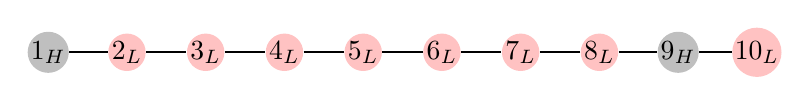
\begin{tikzpicture}[scale=1]
    % Draw a 7,11 network
    % First we draw the vertices
    \foreach \pos/\name in {{(1,0)/1_H}, {(9,0)/9_H}}
        \node[vertex] (\name) at \pos {$\name$};
        
    \foreach \pos/\name in {{(2,0)/2_L}, {(3,0)/3_L}, {(4,0)/4_L}, {(5,0)/5_L}, {(6,0)/6_L}, {(7,0)/7_L}, {(8,0)/8_L}, {(10,0)/10_L}}
    \node[selected vertex] (\name) at \pos {$\name$};
    
    % Connect vertices with edges 
    \foreach \source/ \dest in {1_H/2_L, 2_L/3_L,3_L/4_L,4_L/5_L,5_L/6_L,6_L/7_L, 7_L/8_L,8_L/9_H,9_H/10_L}
        \path[edge] (\source) -- (\dest) ;
        
\end{tikzpicture}
\end{center}

\begin{itemize}
\item There is no chance to learn if $L$-type separate $H$-nodes.
\end{itemize}

  \end{itemize} 

\end{frame}



\begin{frame}
  \frametitle{Repeated Threshold game in network}

$1<s<n$:
  \begin{itemize}
  \item Even there is a chance to learn
\begin{center} 
  
  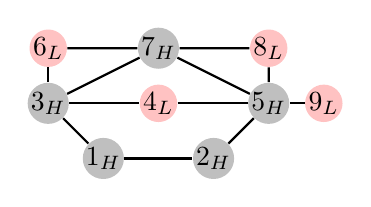
\begin{tikzpicture}[scale=0.7]
    % First we draw the vertices
    \foreach \pos/\name in {{(2,1)/1_H}, {(4,1)/2_H}, {(1,2)/3_H}, {(5,2)/5_H}, {(3,3)/7_H}}
        \node[vertex] (\name) at \pos {$\name$};
        
        \foreach \pos/\name in {{(3,2)/4_L}, {(1,3)/6_L}, {(5,3)/8_L}, {(6,2)/9_L}}
    \node[selected vertex] (\name) at \pos {$\name$};
    
    % Connect vertices with edges 
    \foreach \source/ \dest in {1_H/2_H, 1_H/3_H, 2_H/5_H, 3_H/4_L, 3_H/6_L, 3_H/7_H, 4_L/5_H, 5_H/7_H, 5_H/8_L, 5_H/9_L,6_L/7_H, 7_H/8_L}
        \path[edge] (\source) -- (\dest) ;
\end{tikzpicture}
\end{center}   
  \begin{itemize}
  \item We want to use $\{h,l\}$ to report \textcolor{red}{the correct number} of $H$-nodes.
  \item We also want to use $\{h,l\}$ to \textcolor{red}{report the location} of $H$-nodes.
  \item There is \textcolor{red}{a free-rider problem}: although players' incentives are aligned in the future successfulness,
\begin{itemize}
\item , however they have to take the ``risk'' to report others' types.
\item , however there is a discount if the players can take the risks later.
\end{itemize}  
  
  
  \end{itemize}
  \end{itemize} 
  

\end{frame}






\begin{frame}
  \frametitle{Repeated Threshold game in network}

\begin{definition}
Strong connectivity: For every pair of $H$-type nodes, there is a path consisting $H$-type nodes to connect them.
\end{definition} 

\begin{assumption}
\begin{enumerate}
\item $T$ has strong connectivity
\item The prior: $0<\pi(H)<1$ 
\end{enumerate}

\end{assumption}

\end{frame}


\begin{frame}
  \frametitle{Repeated Threshold game in network}

{\color{red}Main theorem}: There is a class of type spaces in which the revolution can success in the tree networks. 

\begin{theorem}
{\color{red} If} $T$ has strong connectivity, {\color{red} then} for all $0<\pi(H)<1$, for all n-person repeated Threshold game with parameter $1\leq s \leq n$ played in any finite connected undirected network {\color{red} without circle}, there is a $\delta$ such that there is an equilibrium which is approaching efficient.
\end{theorem}


\end{frame}



\begin{frame}
  \frametitle{Conjecture}
  \textcolor{red}{Further goal:}
\begin{conjecture}
{\color{red} If} $T$ has strong connectivity, {\color{red} then} for all $0<\pi(H)<1$, for all n-person repeated Threshold game with parameter $1\leq s \leq n$ played in any finite connected undirected network, there is a $\delta$ such that there is an equilibrium which is approaching efficient.
\end{conjecture}
\end{frame}


\end{document}
